\section{Kadek Diva Krishna Murti}
\subsection{Soal 1}
\textbf{Pengenalan CSV}

Comma Separated Values (CSV) adalah suatu format data yang di mana setiap bagian data dipisahkan dengan tanda koma (,). Format CSV biasanya berfungsi untuk menukar atau mengonversi data ke format lainnya 
%\cite{shafranovich2005common}.

\textbf{Sejarah Format CSV}

IBM Fortran (level H extended) compiler di bawah OS/360 mendukung format CSV pada tahun 1972. FORTRAN 77 mendefinisakan penulisannya dimana input atau output penulisannya menggunakan tanda koma atau spasi untuk pembatas antar data dan penulisan tersebut telah disetujui pada tahun 1978.

Osborne Executive computer yang mengembangkan SuperCalc spreadsheet pada tahun 1983 membuat konvensi kutipan CSV yang memungkinkan string mengandung koma.

Inisiatif standardisasi utama - mentransformasikan "definisi fuzzy de facto" menjadi definisi yang lebih tepat dan de jure - adalah pada tahun 2005, dengan RFC4180, mendefinisikan CSV sebagai Tipe Konten MIME. Kemudian, pada 2013, beberapa kekurangan RFC4180 ditangani oleh rekomendasi W3C.

Pada 2014 IETF menerbitkan RFC7111 yang menjelaskan aplikasi fragmen URI pada dokumen CSV. RFC7111 menentukan bagaimana rentang baris, kolom, dan sel dapat dipilih dari dokumen CSV menggunakan indeks posisi.

Pada 2015 W3C, dalam upaya meningkatkan CSV dengan semantik formal, mempublikasikan draft rekomendasi pertama untuk standar metadata CSV, yang dimulai sebagai rekomendasi pada bulan Desember tahun yang sama.

\textbf{Contoh penggunaan format CSV}

\lstinputlisting[caption = Contoh penggunaan format CSV., firstline=1, lastline=3]{src/4/1174006/Teori/teori.csv}

\subsection{Soal 2}
Aplikasi-aplikasi yang dapat menciptkan file csv, yaitu:

\begin{enumerate}
	\item Editor teks (Notepad, Sublime, Atom, dan lain-lain)
	\item Spreadsheet (Microsoft Excel dan lain-lain)
\end{enumerate}

\subsection{Soal 3}
Cara menulis dan membaca file csv di excel atau spreadsheet, sebagai berikut:

\textbf{Menulis File CSV}

\begin{enumerate}
	\item Pertama silahkan buka aplikasi Excel dengan cara klik ''Start'', cari Excel, kemudian tekan Enter.
	
	\begin{figure}[H]
		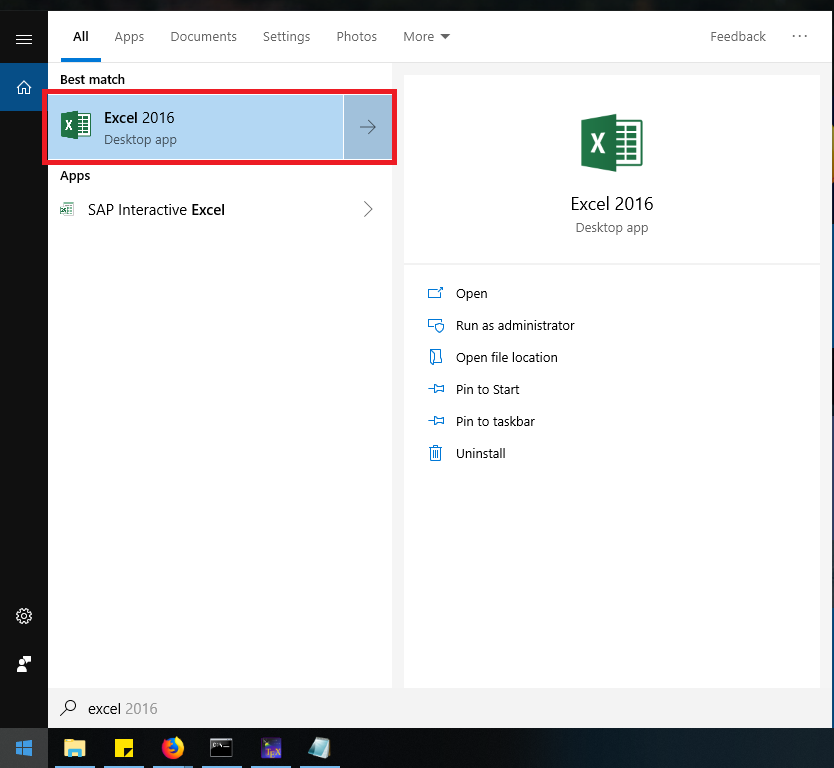
\includegraphics[width=9cm]{figures/4/1174006/Teori/t1.png}
		\centering
	\end{figure}
	
	\item Setelah aplikasi terbuka silahkan klik ''Blank Workbook''.
	
	\begin{figure}[H]
		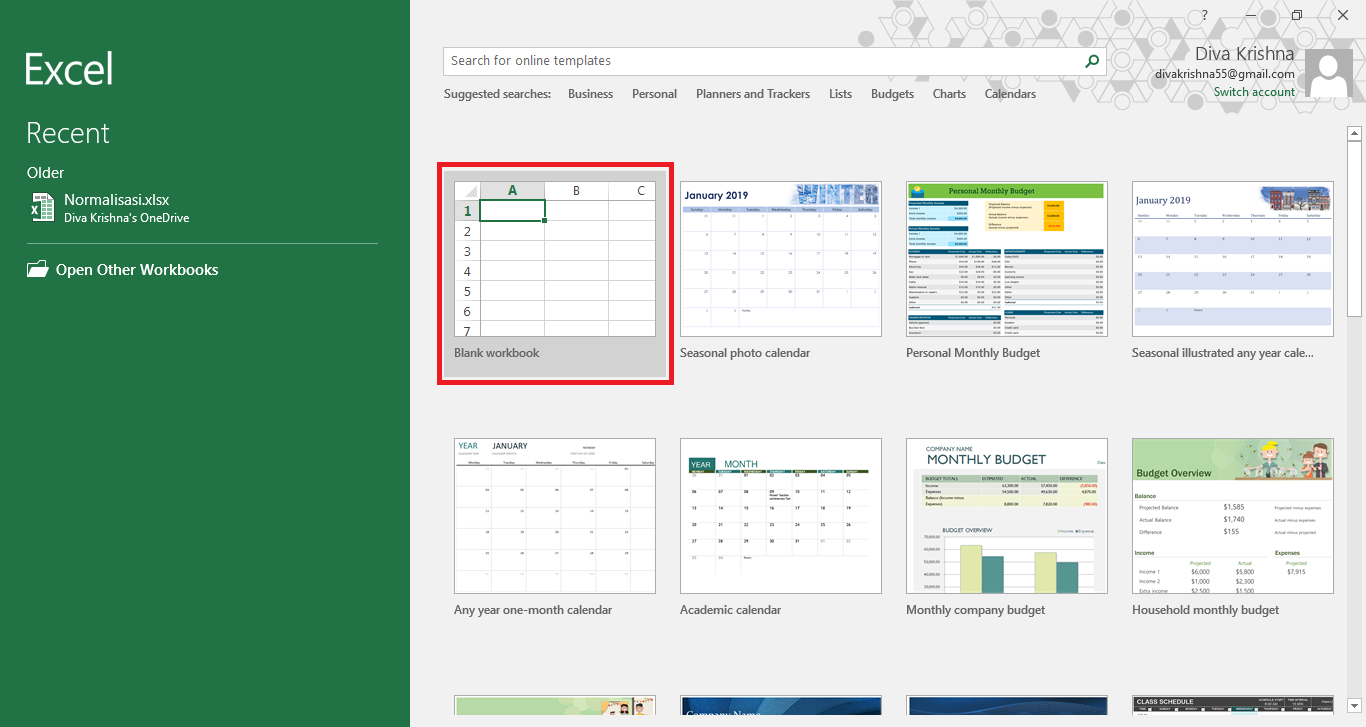
\includegraphics[width=10cm]{figures/4/1174006/Teori/t2.png}
		\centering
	\end{figure}
	
	\item Kemudian isi sesuai dengan data yang ingin dibuat.
	
	\begin{figure}[H]
		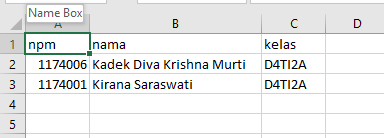
\includegraphics[width=10cm]{figures/4/1174006/Teori/t3.png}
		\centering
	\end{figure}
	
	\item Setelah selesai dibuat, silahkan simpan file tersebut dengan cara mengklik ''File'', lalu klik ''Save''.
	
	\begin{figure}[H]
		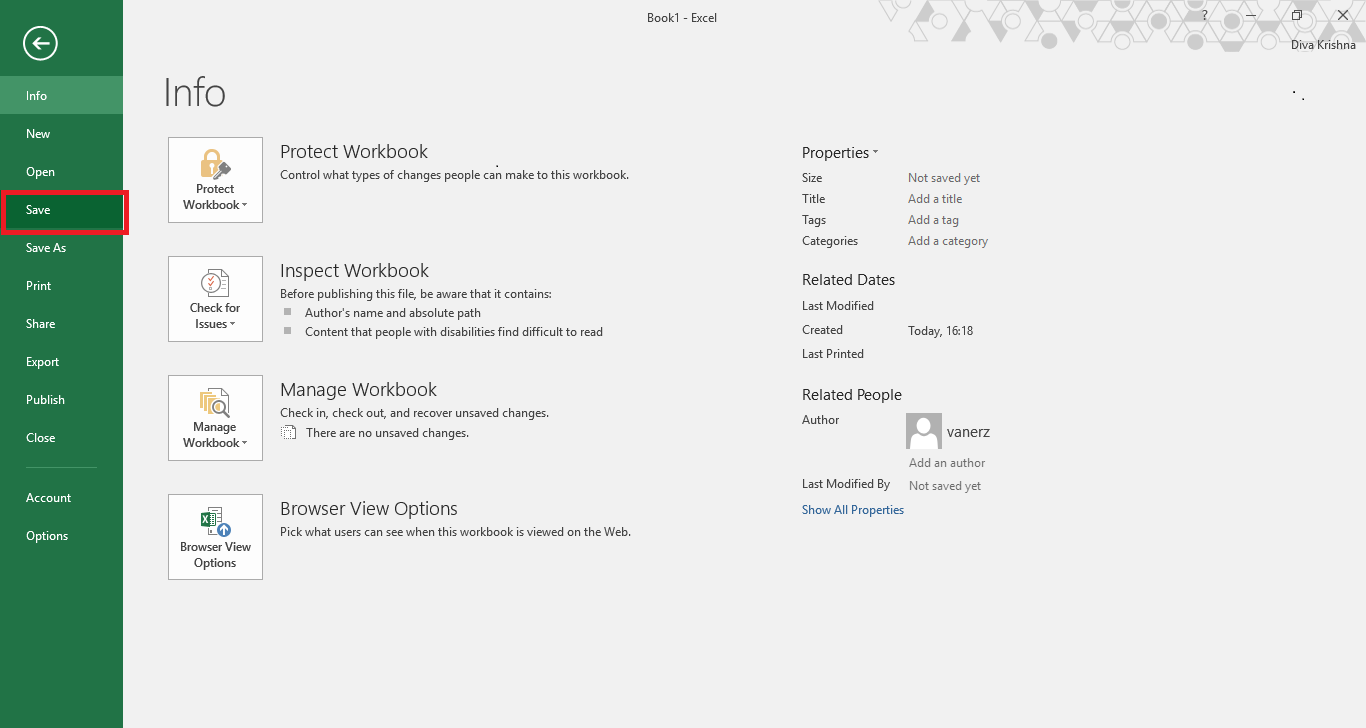
\includegraphics[width=10cm]{figures/4/1174006/Teori/t4.png}
		\centering
	\end{figure}
	
	\item Kemudian isi kolom ''File name'' dengan nama file anda dan kolom ''Save as type'' pilih yang berekstensi .csv.
	
	\begin{figure}[H]
		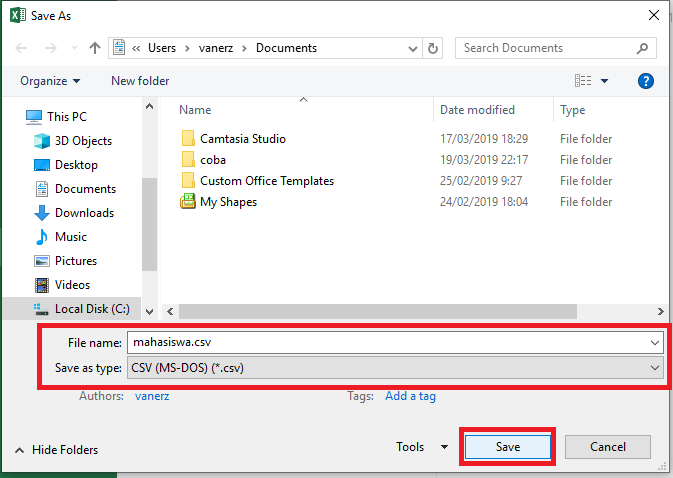
\includegraphics[width=9cm]{figures/4/1174006/Teori/t5.png}
		\centering
	\end{figure}
	
	\item Lalu tinggal klik ''Yes''.
	
	\begin{figure}[H]
		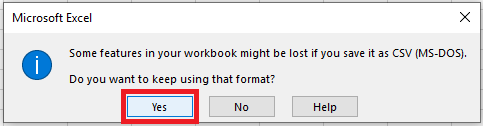
\includegraphics[width=7cm]{figures/4/1174006/Teori/t6.png}
		\centering
	\end{figure}
	
	\item Kemudian file yang Anda telah terbuat tadi tersimpan dengan ekstensi .csv. Untuk melihat isi filenya tinggal klik dua kali pada file tersebut.
	
	\begin{figure}[H]
		
\includegraphics[width=10cm]{figures/4/1174006/Teori/t8.png}
		\centering
	\end{figure}
	
	\item Berikut ini adalah isi dari file yang tadi Anda buat.
	
	\begin{figure}[H]
		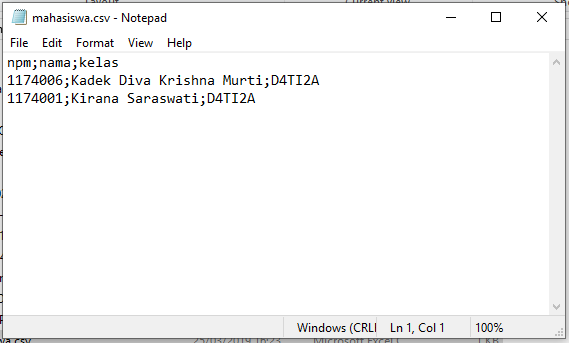
\includegraphics[width=8cm]{figures/4/1174006/Teori/t7.png}
		\centering
	\end{figure}
\end{enumerate}

\textbf{Melihat File CSV di Excel atau Spreadsheet}

\begin{enumerate}
	\item Pertama klik dua kali pada file yang yang berekstensi CSV.
	
	\begin{figure}[H]
		
\includegraphics[width=10cm]{figures/4/1174006/Teori/t8.png}
		\centering
	\end{figure}
	
	\item Kemudian file akan terbuka secara otomatis di aplikasi Excel atau spreadsheet.
	
	\begin{figure}[H]
		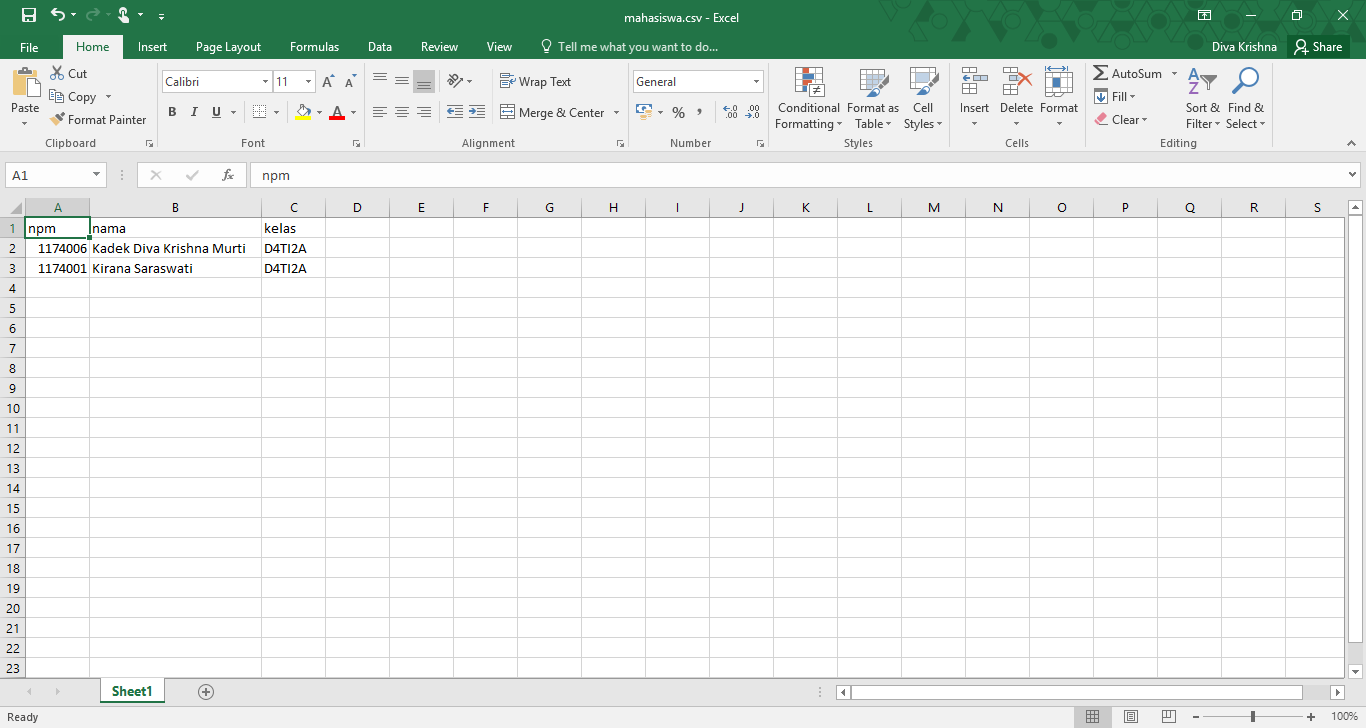
\includegraphics[width=10cm]{figures/4/1174006/Teori/t9.png}
		\centering
	\end{figure}
\end{enumerate}

\subsection{Soal 4}
Sejarah library csv

Library csv mengimplementasikan kelas untuk membaca dan menulis data tabular dalam format CSV. Hal ini memungkinkan programmer untuk mengatakan, "tulis data ini dalam format yang disukai oleh Excel," atau "baca data dari file ini yang dihasilkan oleh Excel," tanpa mengetahui detail yang tepat dari format CSV yang digunakan oleh Excel. Pemrogram juga dapat menggambarkan format CSV yang dipahami oleh aplikasi lain atau menentukan format CSV tujuan khusus mereka sendiri.

\subsection{Soal 5}
Sejarah library pandas

Pada 2008, pengembangan pandas dimulai di AQR Capital Management. Pada akhir 2009 telah menjadi open source, dan secara aktif didukung hari ini oleh komunitas individu yang berpikiran sama di seluruh dunia yang menyumbangkan waktu dan energi berharga mereka untuk membantu membuat panda open source menjadi mungkin.

Sejak 2015, pandas adalah proyek yang disponsori NumFOCUS. Ini akan membantu memastikan keberhasilan pengembangan panda sebagai proyek sumber terbuka kelas dunia.

\subsection{Soal 6}
Fungsi-fungsi yang terdapat di library csv, yaitu:
\begin{enumerate}
	\item reader
	
	Fungsi ini digunakan untuk membaca isi file berformat CSV dari list.
	
	\lstinputlisting[caption = Membaca file berformat CSV list., firstline=7, lastline=13]{src/4/1174006/Teori/1174006.py}
	
	\item DictReader
	
	Fungsi ini digunakan untuk membaca isi file berformat CSV dari dictionary.
	
	\lstinputlisting[caption =  Membaca file berformat CSV dictionary., firstline=15, lastline=21]{src/4/1174006/Teori/1174006.py}
	
	\item write
	
	Fungsi ini digunakan untuk menulis file berformat CSV dari list.
	
	\lstinputlisting[caption =  Menulis file berformat CSV list., firstline=23, lastline=30]{src/4/1174006/Teori/1174006.py}
	
	\item DictWrite
	
	Fungsi ini digunakan untuk menulis file berformat CSV dari dictionary.
	
	\lstinputlisting[caption =  Menulis file berformat CSV dictionary., firstline=32, lastline=41]{src/4/1174006/Teori/1174006.py}
	
\end{enumerate}

\subsection{Soal 7}
Fungsi-fungsi yang terdapat di library pandas, yaitu:
\begin{enumerate}
	\item read\_csv
	
	Fungsi ini digunakan untuk membaca isi file berformat CSV
	
	\lstinputlisting[caption =  Membaca file berformat CSV pandas., firstline=43, lastline=47]{src/4/1174006/Teori/1174006.py}
	
	\item to\_csv
	
	Fungsi ini digunakan untuk menulis file berformat CSV
	
	\lstinputlisting[caption =  Menulis file berformat CSV pandas., firstline=49, lastline=53]{src/4/1174006/Teori/1174006.py}
	
\end{enumerate}

\subsection{Kode Program Teori}
\begin{figure}[H]
	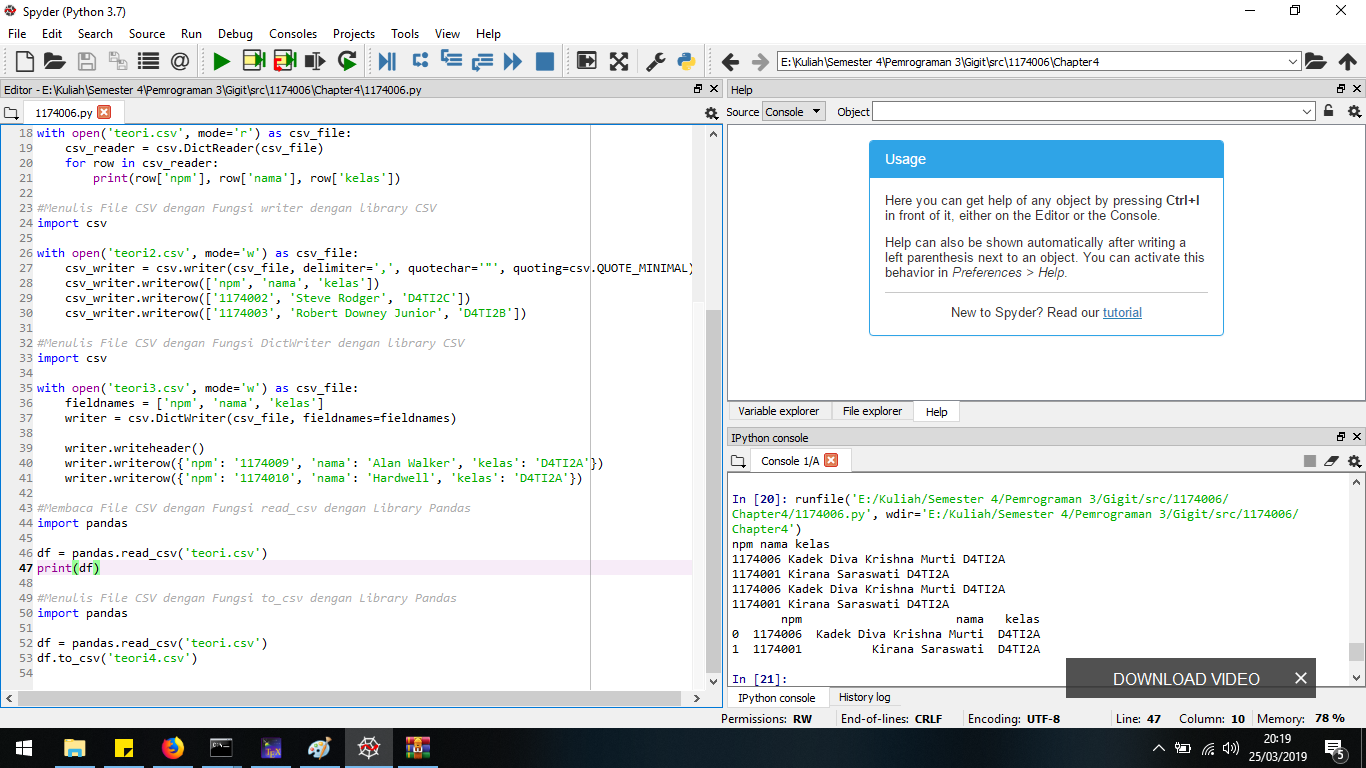
\includegraphics[width=10cm]{figures/4/1174006/Teori/kode_teori1.png}
	\centering
\end{figure}

\begin{figure}[H]
	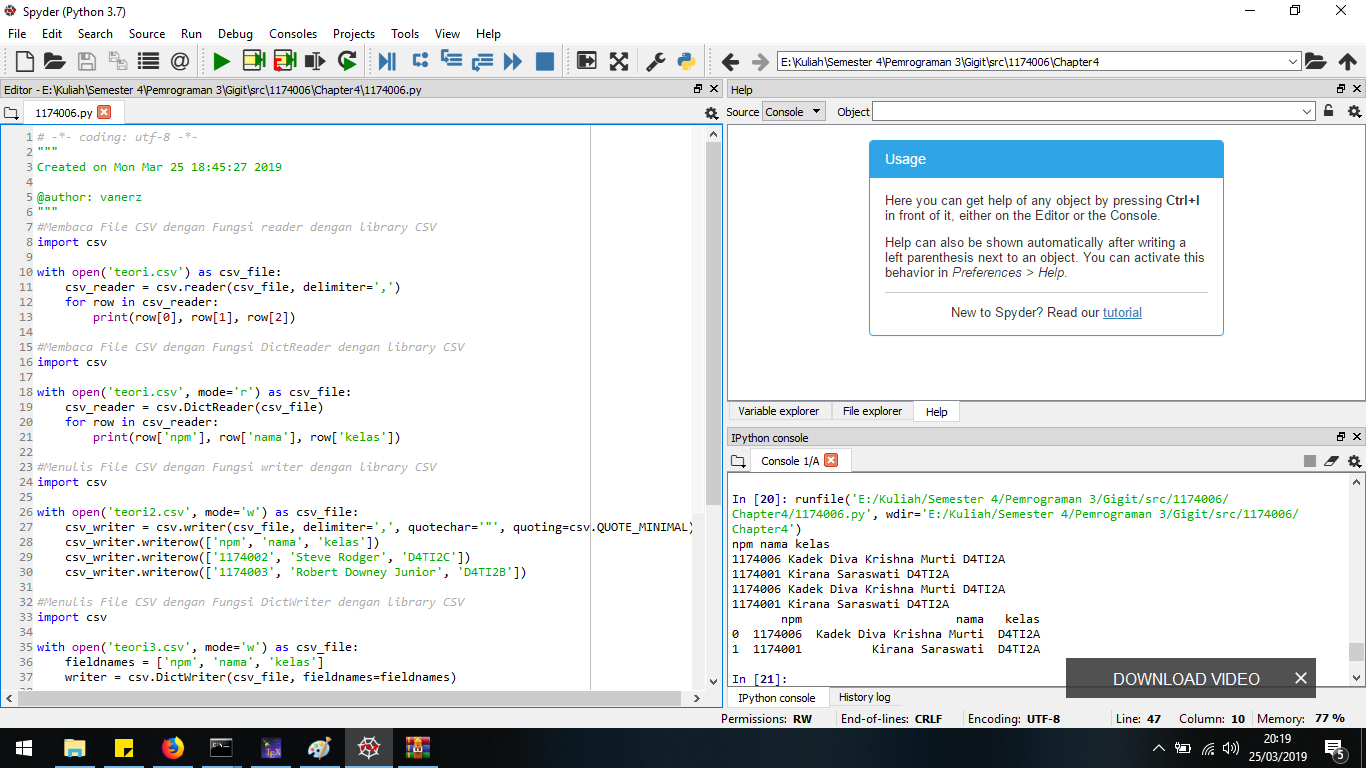
\includegraphics[width=10cm]{figures/4/1174006/Teori/kode_teori2.png}
	\centering
\end{figure}

\subsection{Cek Plagiat Teori}

\begin{figure}[H]
	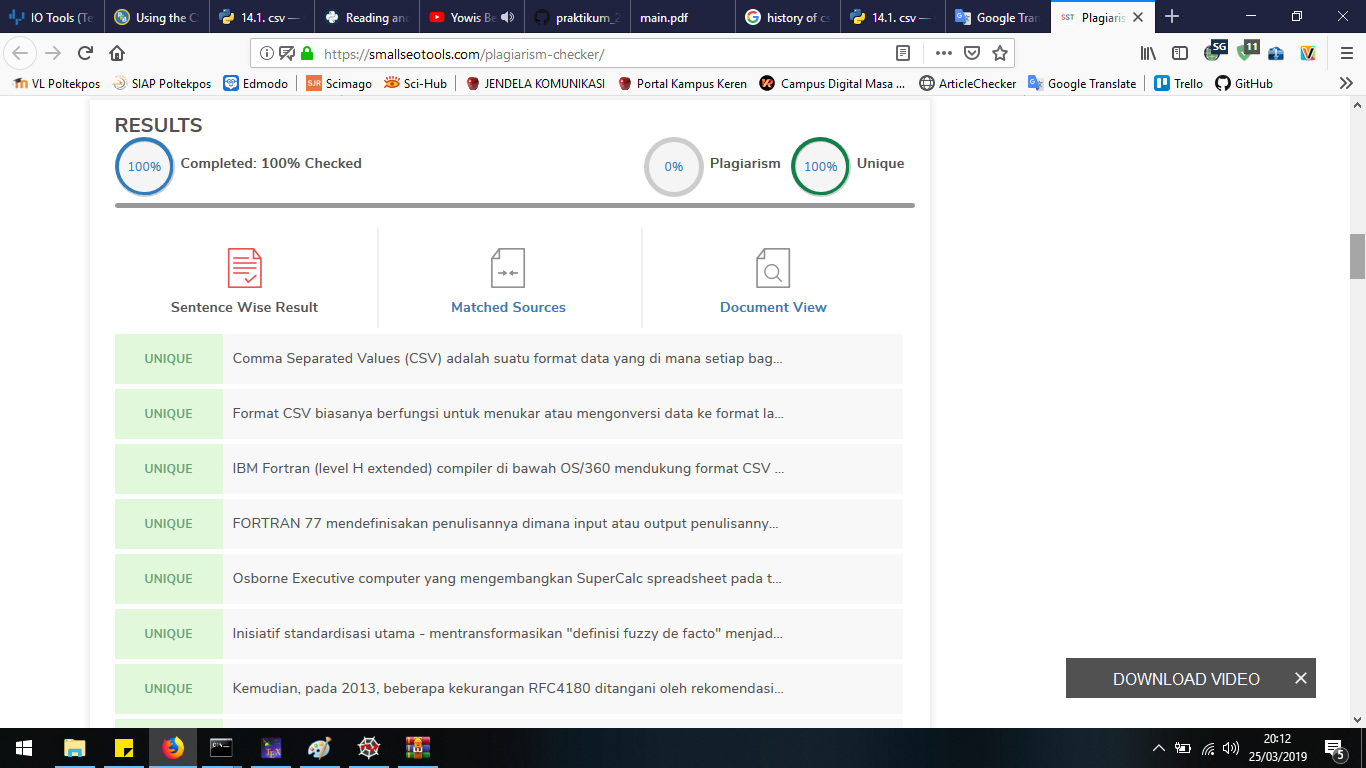
\includegraphics[width=10cm]{figures/4/1174006/Teori/plagiat_teori.png}
	\centering
\end{figure}


\section{Dwi Yulianingsih}
\subsection{Soal 1}
Isi jawaban soal ke-1

Kalau mau dibikin paragrap \textbf{cukup enter aja}, tidak usah pakai \verb|par| dsb

%\subsection{Soal 2}
%Isi jawaban soal ke-2

%\subsection{Soal 3}
%Isi jawaban soal ke-3

\section{Harun Ar-Rasyid}
\subsection{Soal 1}
Isi jawaban soal ke-1

Kalau mau dibikin paragrap \textbf{cukup enter aja}, tidak usah pakai \verb|par| dsb

%\subsection{Soal 2}
%Isi jawaban soal ke-2

%\subsection{Soal 3}
%Isi jawaban soal ke-3

\section{Sri Rahayu}
\subsection{Soal 1}
Isi jawaban soal ke-1

Kalau mau dibikin paragrap \textbf{cukup enter aja}, tidak usah pakai \verb|par| dsb

%\subsection{Soal 2}
%Isi jawaban soal ke-2

%\subsection{Soal 3}
%Isi jawaban soal ke-3

\section{Doli Jonviter}
\subsection{Soal 1}
Isi jawaban soal ke-1

Kalau mau dibikin paragrap \textbf{cukup enter aja}, tidak usah pakai \verb|par| dsb

%\subsection{Soal 2}
%Isi jawaban soal ke-2

%\subsection{Soal 3}
%Isi jawaban soal ke-3

\section{Rahmatul Ridha}
\subsection{Soal 1}
Isi jawaban soal ke-1

Kalau mau dibikin paragrap \textbf{cukup enter aja}, tidak usah pakai \verb|par| dsb

%\subsection{Soal 2}
%Isi jawaban soal ke-2

%\subsection{Soal 3}
%Isi jawaban soal ke-3

\section{Tomy Prawoto}
\subsection{Soal 1}
Isi jawaban soal ke-1

Kalau mau dibikin paragrap \textbf{cukup enter aja}, tidak usah pakai \verb|par| dsb

%\subsection{Soal 2}
%Isi jawaban soal ke-2

%\subsection{Soal 3}
%Isi jawaban soal ke-3
